\chapter*{Appendix}\label{chapter:appendix}
\phantomsection\addcontentsline{toc}{chapter}{Appendix}

\begin{table}[H]
\centering
\caption{Accumulated measurements for each experiment in Swarm without outliers.}
\resizebox{\textwidth}{!}{%
\begin{tabular}{@{}lcccccccc@{}}
\toprule
Experiment    & \multicolumn{7}{c}{Data Size}          & Failures (\%) \\ \midrule
& 4kb  & 16kb  & 64kb  & 256kb  & 1mb  & 4mb  & 16mb              \\ \midrule
simple & 35.91 & 207.6 & 302.56 & 475.75 & 1126.42 & 3727.21 & 9815.11 & 9 \\
no-cache  & 50.49 & 258.35 & 314.25 & 467.14 & 1206.17 & 3418.18 & 8391.32 & 9 \\
disconnect  & 52.21 & 179.63 & 344.74 & 467.44 & 1247.89 & 3507.51 & 8713.88 & 7 \\
no-cache-disconnect  & 51.54 & 152.27 & 327.29 & 441.47 & 1208.57 & 3497.87 & 8567 & 10 \\
\bottomrule
\end{tabular}
}
\end{table}


\begin{table}[H]
\centering
\begin{small}
\caption{Accumulated measurements for each experiment in IPFS without outliers.}
\resizebox{\textwidth}{!}{%
\begin{tabular}{@{}lcccccccc@{}}
\toprule
Experiment    & \multicolumn{7}{c}{Data Size}          & Failures (\%) \\ \midrule
& 4kb  & 16kb  & 64kb  & 256kb  & 1mb  & 4mb  & 16mb              \\ \midrule
simple & 199.88 & 154.76 & 171.33 & 194.54 & 212.07 & 402.53 & 1209.93 & 4 \\
no-cache  & 160.85 & 51.96 & 72.66 & 97.88 & 116.75 & 195.59 & 638.54 & 24 \\
disconnect  & 135.36 & 124.72 & 1168.58 & 310.82 & 1360.46 & 469.56 & 1275.26 & 37 \\
no-cache-disconnect  & 151.11 & 163.59 & 263.22 & 313.85 & 1758.96 & 759.66 & 1801.96  & 53 \\
\bottomrule
\end{tabular}
}
\end{small}
\end{table}


\begin{table}[H]
\centering
\begin{small}
\caption{Accumulated measurements for each experiment in IPFS without outliers (degroot-miletus-nancy).}
\label{tab:miletus_degroot_nancy}
\resizebox{\textwidth}{!}{%
\begin{tabular}{@{}lcccccccc@{}}
\toprule
Experiment    & \multicolumn{7}{c}{Data Size}          & Failures (\%) \\ \midrule
& 4kb  & 16kb  & 64kb  & 256kb  & 1mb  & 4mb  & 16mb              \\ \midrule
simple & 188.38 & 149.39 & 158.54 & 167.08 & 292.41 & 461.01 & 1816.65 & 0 \\
no-cache  & 146.06 & 141.99 & 143.93 & 152.68 & 261.62 & 524.04 & 1955.46 & 3 \\
disconnect  & 189.47 & 306.23 & 1252.18 & 1281.77 & 1751.59 & 1458.82 & 3536.62 & 12 \\
no-cache-disconnect  & 198.14 & 170.18 & 1230.74 & 372.82 & 1961.7 & 2011.86 & 3162.53 & 27 \\
\bottomrule
\end{tabular}
}
\end{small}
\end{table}

\begin{table}[H]
\centering
\begin{small}
\caption{Accumulated measurements for IPFS without outliers.}
\begin{tabular}{@{}lccccccc@{}}
\toprule
Size & Mean & Median & Skewness & Min & Max & Sample Size & Outliers \\ \midrule
4KB & 146.85 & 145.64 & 0.31 & 6.99 & 394.83 & 326 & 89\\
16KB & 113.8 & 141.63 & -0.32 & 3.13 & 243.88 & 328 & 62\\
64KB & 153.98 & 158.9 & 0.67 & 3.32 & 655.62 & 295 & 89\\
256KB & 210.55 & 174.56 & 1.4 & 38.86 & 891.33 & 318 & 82\\
1MB & 737.98 & 310.51 & 1.49 & 9.67 & 3600.76 & 391 & 19\\
4MB & 564.25 & 415.7 & 1.82 & 99.65 & 2399.45 & 363 & 49\\
16MB & 1359.79 & 1216.78 & 1.21 & 297.5 & 4592.43 & 369 & 29\\
\bottomrule
\end{tabular}
\end{small}
\end{table}

\begin{table}[H]
\centering
\begin{small}
\caption{Accumulated measurements for Swarm without outliers.}
\begin{tabular}{@{}lccccccc@{}}
\toprule
Size & Mean & Median & Skewness & Min & Max & Sample Size & Outliers \\ \midrule
4KB & 43.66 & 50.49 & 0.74 & 1.19 & 182.76 & 356 & 39\\
16KB & 218.75 & 196.73 & 0.58 & 2.66 & 662.08 & 389 & 6\\
64KB & 330.4 & 319.61 & 0 & 3.32 & 677.07 & 380 & 15\\
256KB & 483.43 & 465.3 & 0.04 & 4.69 & 978.37 & 381 & 14\\
1MB & 1276.7 & 1217.82 & 0.65 & 675.32 & 2259.57 & 378 & 22\\
4MB & 3623.02 & 3520.14 & 0.5 & 2165.56 & 5889.15 & 387 & 17\\
16MB & 9037.03 & 8914.55 & 0.46 & 5822.69 & 14261.94 & 159 & 10\\
\bottomrule
\end{tabular}
\end{small}
\end{table}






% \begin{table}[H]
% \centering
% \begin{small}
% \caption{Accumulated measurements for experiment \textit{simple} in IPFS. The dataset consists of 1050 samples in total (including failures), with retrieval failure ratio of $\sim 4\%$ }
% \label{tab:simple_dirty}
% \begin{tabular}{@{}lccccccc@{}}
% \toprule
% Size & Mean & Median & IQR & Skewness & Min & Max & Sample Size \\ \midrule
% 4KB & 472.96 & 211.66 & 109.01 & 3.69 & 30.04 & 5408.44 & 140\\
% 16KB & 135.24 & 150.64 & 28.92 & -1.06 & 30.90 & 203.29 & 143\\
% 64KB & 176.44 & 175.63 & 90.05 & -0.19 & 34.75 & 382.46 & 143\\
% 256KB & 247.11 & 239.92 & 161.51 & 1.17 & 38.85 & 712.93 & 145\\
% 1MB & 514.83 & 234.93 & 202.04 & 11.63 & 52.27 & 27258.04 & 146\\
% 4MB & 635.02 & 431.22 & 246.71 & 2.64 & 103.36 & 3260.39 & 145\\
% 16MB & 1797.22 & 1306.89 & 688.50 & 2.70 & 338.36 & 9525.16 & 144\\
% \bottomrule
% \end{tabular}
% \end{small}
% \end{table}

% \begin{table}[H]
% \centering
% \begin{small}
% \caption{Accumulated measurements for experiment \textit{disconnect} in IPFS. The dataset consists of 665 samples in total (including failures), with retrieval failure ratio of $\sim 6.5\%$ }
% \label{tab:disconnect}
% \begin{tabular}{@{}lccccccc@{}}
% \toprule
% Size & Mean & Median & IQR & Skewness & Min & Max & Sample Size \\ \midrule
% 4KB & 899.4 & 144.2 & 1040.53 & 2.14 & 6.99 & 8551.52 & 141\\
% 16KB & 1234.05 & 139.67 & 1051.18 & 5.94 & 3.13 & 29803.37 & 128\\
% 64KB & 2417.38 & 1264.5 & 2557.39 & 3.92 & 3.32 & 29352.31 & 123\\
% 256KB & 1474.87 & 335.85 & 1385.74 & 6.63 & 42.83 & 30001.96 & 130\\
% 1MB & 1431.46 & 1360.46 & 2015.44 & 0.83 & 9.67 & 5071.64 & 136\\
% 4MB & 1783.34 & 494.24 & 1737.18 & 5.14 & 99.65 & 27082.3 & 139\\
% 16MB & 2184.65 & 1363.14 & 2050.4 & 5.38 & 297.5 & 26714.33 & 133\\
% \bottomrule
% \end{tabular}
% \end{small}
% \end{table}



\begin{table}[H]
\centering
\begin{small}
\caption{IPFS: accumulated measurements for our machine (degroot). The dataset consists of 665 samples in total (including failures), with retrieval failure ratio of $\sim 6.5\%$ }
\label{tab:degroot_ipfs}
\begin{tabular}{@{}lcccccc@{}}
\toprule
Size & Mean & Median & Skewness & Min & Max & Sample Size \\ \midrule
4KB & 1421.16 & 242.18 & 1.18 & 139.82 & 5819.67 & 88\\
16KB & 1065.02 & 170.23 & 2.54 & 128.68 & 10072.69 & 86\\
64KB & 1308.95 & 249.04 & 3.58 & 131.93 & 14766.25 & 87\\
256KB & 981.47 & 313.59 & 1.89 & 143.75 & 5293.09 & 90\\
1MB & 1249.65 & 385.42 & 1.22 & 195.49 & 5071.64 & 89\\
4MB & 1799.89 & 516.34 & 4.38 & 337.33 & 21345.4 & 93\\
16MB & 2476.33 & 1499.17 & 1.72 & 995.34 & 9461.04 & 89\\
\bottomrule
\end{tabular}
\end{small}
\end{table}

\begin{table}[H]
\centering
\begin{small}
\caption{IPFS: accumulated measurements for Lille site. The dataset consists of 665 samples in total (including failures), with retrieval failure ratio of $\sim 44\%$ }
\begin{tabular}{@{}lcccccc@{}}
\toprule
Size & Mean & Median & Skewness & Min & Max & Sample Size \\ \midrule
4KB & 556.61 & 130.76 & 5.58 & 33.68 & 10806.75 & 56\\
16KB & 199.35 & 123.73 & 4.32 & 28.48 & 2182.87 & 51\\
64KB & 485.99 & 175.87 & 2.23 & 40.17 & 3269.44 & 52\\
256KB & 491.22 & 201.17 & 2.25 & 49.33 & 3402.34 & 52\\
1MB & 1325.06 & 272.27 & 6.46 & 58.97 & 27258.05 & 55\\
4MB & 1298.11 & 464.68 & 6.03 & 108.31 & 22407.71 & 54\\
16MB & 1618.79 & 1098.98 & 2.91 & 304.16 & 9793.04 & 52\\
\bottomrule
\end{tabular}
\end{small}
\end{table}

\begin{table}[H]
\centering
\begin{small}
\caption{Swarm: accumulated measurements for our machine (degroot). The dataset consists of 458 samples in total (including failures), with retrieval failure ratio of $\sim 9\%$ }
\begin{tabular}{@{}lcccccc@{}}
\toprule
Size & Mean & Median & Skewness & Min & Max & Sample Size \\ \midrule
4KB & 125.64 & 106.78 & 1.13 & 1.19 & 375.95 & 65\\
16KB & 355.39 & 356.69 & 0.35 & 6.21 & 731.93 & 65\\
64KB & 506.36 & 455.06 & 0.8 & 6.14 & 1034.46 & 65\\
256KB & 701.1 & 659.04 & 0.52 & 10.05 & 1484.6 & 65\\
1MB & 1752.64 & 1718.43 & -0.5 & 16.36 & 2673.54 & 65\\
4MB & 4703.53 & 4606.77 & -1.05 & 39.54 & 7884.58 & 66\\
16MB & 12671.97 & 11706.08 & 0.8 & 8623.28 & 18851.85 & 25\\
\bottomrule
\end{tabular}
\end{small}
\end{table}

\begin{table}[H]
\centering
\begin{small}
\caption{Swarm: accumulated measurements for Lille site. The dataset consists of 474 samples in total (including failures), with retrieval failure ratio of $\sim 8\%$ }
\begin{tabular}{@{}lcccccc@{}}
\toprule
Size & Mean & Median & Skewness & Min & Max & Sample Size \\ \midrule
4KB & 31.59 & 31.63 & 4.54 & 2.41 & 398.32 & 67\\
16KB & 129.7 & 62.44 & 1.51 & 3.38 & 515.84 & 67\\
64KB & 262.84 & 267.23 & 0.09 & 3.72 & 588.63 & 67\\
256KB & 384.88 & 365.31 & 0.45 & 5.01 & 811.72 & 67\\
1MB & 991.81 & 976.45 & -0.61 & 10.82 & 1796.9 & 68\\
4MB & 2874.76 & 2855.04 & -1.46 & 34.05 & 4680.03 & 68\\
16MB & 8463.23 & 8544.81 & -0.14 & 5822.69 & 10991.23 & 30\\
\bottomrule
\end{tabular}
\end{small}
\end{table}







% \begin{figure}[htbp]
% \centerline{\includegraphics[width=\textwidth]{figs/degroot_disconnect_box_plot.png}}
% \caption{.}
% \label{fig:degroot_disconnect_box_plot}
% \end{figure}


\begin{table}[]
    \caption{Accumulated measurements for the hosts participating in the experiments (IPFS).}
\resizebox{\textwidth}{!}{%
\begin{tabular}{@{}lclllllllllllllcc@{}}
\toprule
Host & \multicolumn{14}{c}{Data Size}                                                                                                                                                                                                                                                                                                               & \multicolumn{2}{c}{Failures (\%)}        \\ \midrule
     & \multicolumn{2}{c}{-----4kb-----}                         & \multicolumn{2}{c}{   16kb   }                          & \multicolumn{2}{c}{64kb}                          & \multicolumn{2}{c}{256kb}                          & \multicolumn{2}{c}{1mb}                          & \multicolumn{2}{c}{4mb}                          & \multicolumn{2}{c}{16mb}                          &             &         \\ \midrule
     &       \multicolumn{1}{c}{I}              & \multicolumn{1}{c}{S} & \multicolumn{1}{c}{I} & \multicolumn{1}{c}{S} & \multicolumn{1}{c}{I} & \multicolumn{1}{c}{S} & \multicolumn{1}{c}{I} & \multicolumn{1}{c}{S} & \multicolumn{1}{c}{I} & \multicolumn{1}{c}{S} & \multicolumn{1}{c}{I} & \multicolumn{1}{c}{S} & \multicolumn{1}{c}{I} & \multicolumn{1}{c}{S} &           \multicolumn{1}{c}{I} & \multicolumn{1}{c}{S}           \\ \midrule
 degroot   & 242 & 106 & 170 & 356 & 249 & 455 & 313 & 659 & 385 & 1718 & 516 & 4606 & 1499 & 11706 & 6.5 & 9 \\
 nancy     & 144 & 50  & 140 & 121 & 153 & 302 & 155 & 422 & 306 & 1141 & 376 & 3220 & 1095 & 7399  & 21  & 9 \\
 lille     & 130 & 31  & 123 & 62  & 175 & 267 & 201 & 365 & 272 & 976  & 464 & 2855 & 1098 & 8544  & 44 & 8 \\
 grenoble  & 143 & 52  & 142 & 185 & 157 & 312 & 168 & 476 & 304 & 1183 & 389 & 3485 & 997  & 9405  & 36 & 8 \\
 rennes    & 147 & 53  & 134 & 129 & 151 & 313 & 166 & 439 & 198 & 1056 & 409 & 3412 & 944  & 8631  & 31 & 8 \\
 sophia    & 159 & 62  & 153 & 266 & 198 & 339 & 216 & 510 & 243 & 1244 & 449 & 3528 & 1331 & 9677  & 38 & 9 \\
\bottomrule
\end{tabular}
}
\end{table}


\begin{figure}[htbp]
\centerline{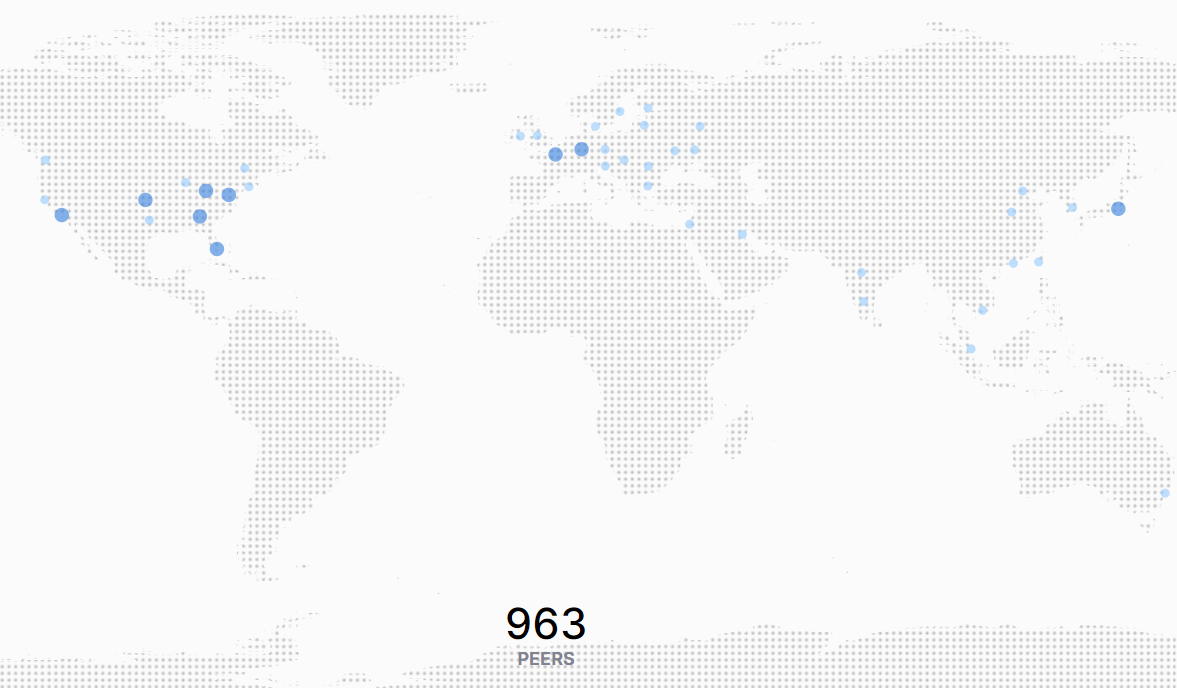
\includegraphics[width=\textwidth]{figs/ipfs_peers.png}}
\caption{Geographical distribution of connected peers in IPFS.}
\label{fig:ipfs_peers}
\end{figure}
